\documentclass{article}
\usepackage[bottom=2cm, right=1.5cm, left=1.5cm, top=2cm]{geometry}
\usepackage{amsmath}
\usepackage{amssymb}
\usepackage{amsthm}
\usepackage{enumitem}
\usepackage{exercise} % Exercises Style
\usepackage{graphicx}
\usepackage{caption}
\usepackage{environ}

% Enable Code
\usepackage{minted}
\let \extra T
\newcommand{\vect}[1]{\boldsymbol{#1}}
\newcommand{\vectrm}[1]{\boldsymbol{\rm #1}}
\DeclareMathOperator{\Tr}{Tr}
\DeclareMathOperator{\Cov}{Cov}
\DeclareMathOperator{\Var}{Var}
\DeclareMathOperator{\E}{E}
\DeclareMathOperator{\diag}{diag}

\usepackage{fancyhdr}
\newenvironment{solution}
{\renewcommand\qedsymbol{$\blacksquare$}
\begin{proof}[Solution]$ $}
  {
\end{proof}}

\title{Solutions to Exam 1 }
\author{Rongfei Jin}
\begin{document}

\pagestyle{fancy}
\fancyhf{}%
\fancyhead[L]{\textbf{ DS5220 \ Exam 1 }}
\fancyhead[R]{\textbf{Rongfei Jin}}
\fancyfoot[C]{\thepage}%
\bibliographystyle{plain} 
\maketitle

\section*{Problem 1}
\begin{enumerate}[label=(\alph*)]
  \item See (Appendix 1)
  \item See (Appendix 1) \\
  Some values are NA in the summary because of the collinearity which means that the design matrix is not full rank
  \item
    \begin{enumerate}[label=(\arabic*)]

      \item Gender
        \begin{enumerate}[label=(\roman*)]
          \item Faster multiplication on 0
          \item
            gender encoded in 0,1 is easiser to interpret because the coefficients represents the effect of being male, or no effect if being female
        \end{enumerate}
      \item Income and travel


        inc25p: 1 if income is greater than 25k, 0 otherwise \\
        inc55p: 1 if income is greater than 55k, 0 otherwise \\
        inc95p: 1 if income is greater than 95k, 0 otherwise \\
        tra025p: 1 if travel is greater than .25h, 0 otherwise \\
        tra400p: 1 if travel is greater than 4h, 0 otherwise \\

        \begin{enumerate}[label=(\roman*)]
          \item Design matrix achieves full rank.
            These transformations solve the collinearity problem since if the model has all the condition except the last one, then the last one is determined, so numerically it is more stable.

          \item
            Easier to interpret as the coefficients are simply the effect of income greater than a certain threshold

        \end{enumerate}
    \end{enumerate}

  \item
      \begin{figure}[h]
          \centering
          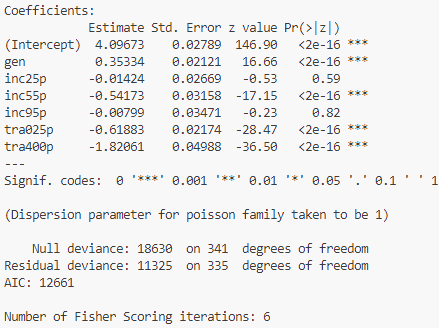
\includegraphics[width=0.5\textwidth]{1d.png}
          \caption{Model 1d}
      \end{figure}
    The new model has 7 coefficients (without intercept) and NO coefficients are NA. Gender, income greater than 55k, travel time greater than 0.25h and travel time greater than 4h are significant. \\

    Based on the significant coefficients, we can make the following interpretation.

    \begin{enumerate}[label=(\roman*)]
      \item Males are associated with 0.36 more visit than female
      \item Income greater than 55k is associated with 0.5 less visit than income less than 55k
      \item Travel time greater than 0.25h is associated with 0.6 less visit than travel time less than 0.25h
      \item Travel time greater than 4h is associated with 1.8 less visit than travel time less than 4h

    \end{enumerate}
  
  \item
  \begin{figure}[h]
      \centering
      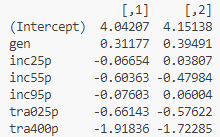
\includegraphics[width=0.5\textwidth]{1e.png}
      \caption{Model CI}
  \end{figure}
  \item
    The possion regression has the following probability density function
    \[
      p(y|\eta) = \frac{\eta^y e^{-\eta}}{y!}
    \]
    where $\eta = \exp(\beta_0 + \beta_1 X_1 + \ldots + \beta_p X_p)$ is the mean of the possion distribution. Therefore, we have
    \[
      \E(y|x_1, \ldots, x_p) = \eta = \exp(\beta_0 + \beta_1 x_1 + \ldots + \beta_p x_p)
    \]

    Given female, earning \(\$\)65,000 annually, and living two miles from the park (We assume the travel time will be less than 0.25h given minimal speed 40mph). We have the following data
    \(\text{gen} = 0\), \(\text{inc25p} = 1\) \(\text{inc55p} = 1\), \(\text{inc95p} = 0\),\(\text{tra025p} = 0\), \(\text{tra400p} = 0\).

    Therefore, we have
    \[
      \E(y|x_1, \ldots, x_p) = \exp(\beta_0 + \beta_1 0 + \beta_2 1 + \beta_3 1 + \beta_4 0 + \beta_5 0 + \beta_6 0) = \exp(\beta_0 + \beta_2 + \beta_3) = 34.49
    \]
    Given male, earning \(\$\)65,000 annually, and living two miles from the park. We have the following data

    \(\text{gen} = 1\), \(\text{inc25p} = 1\) \(\text{inc55p} = 1\), \(\text{inc95p} = 0\),\(\text{tra025p} = 0\), \(\text{tra400p} = 0\).

    \[
      \E(y|x_1, \ldots, x_p) = \exp(\beta_0 + \beta_1 1 + \beta_2 1 + \beta_3 1 + \beta_4 0 + \beta_5 0) = \exp(\beta_0 + \beta_1 + \beta_2 + \beta_3) = 49.11
    \]

    \[\frac{E(y|\text{male with given conditions})}{E(y|\text{female with given conditions})} = \frac{49.11}{34.49} \approx 1.42\]

    \[\frac{E(y|\text{female with given conditions})}{E(y|\text{male with given conditions})} = \frac{34.49}{49.11} \approx 0.703\]

\end{enumerate}

\newpage
\section*{Problem 2}

\begin{enumerate}[label=(\alph*)]
  \item See (Appendix 2)
  \begin{figure}[h]
      \centering
      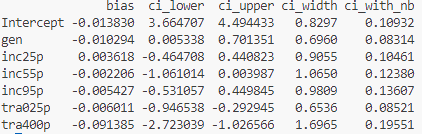
\includegraphics[width=0.5\textwidth]{2a.png}
      \caption{Bootstrap CI}
  \end{figure}
  \item
    \begin{enumerate}[label=(\roman*)]
      \item the center from both approaches are very close
      \item the bootstrapped CI width is wider than the normal CI, which is expected since the normal CI assumes the distribution is normal, but the bootstrapped CI does not make this assumption

    \end{enumerate}
\end{enumerate}

\newpage
\section*{Problem 3}
\begin{enumerate}[label=(\alph*)]
  \item

    Since \(Y \sim \text{Poisson}(\lambda)\) we have
    \(P(Y=y;\lambda) = \frac{\lambda^y e^{-\lambda}}{y!}\)

    We compute the Momement Generating Function
    \begin{align*}
      M_Y(t) &= \E(e^{tY}) \\
      &= \sum_{y=0}^{\infty} e^{ty} P(Y=y;\lambda) \\
      &= \sum_{y=0}^{\infty} e^{ty} \frac{\lambda^y e^{-\lambda}}{y!} \\
      &= e^{-\lambda} \sum_{y=0}^{\infty} \frac{(\lambda e^t)^y}{y!} \\
      &= e^{-\lambda} e^{\lambda e^t} & \text{Taylor expansion}\\
      &= e^{\lambda (e^t - 1)}
    \end{align*}
    Now we compute mean by deriving the first moment
    \begin{align*}
      \E(Y) &= M_Y'(0) \\
      &= \frac{d}{dt} e^{\lambda (e^t - 1)} \bigg|_{t=0} \\
      &= \lambda e^{\lambda (e^0 - 1)} \\
      &= \lambda
    \end{align*}

    Now we compute the variance by first deriving the second moment
    \begin{align*}
      \E(Y^2) &= M_Y''(0) \\
      &= \frac{d^2}{dt^2} e^{\lambda (e^t - 1)} \bigg|_{t=0} \\
      &= \lambda e^{\lambda (e^0 - 1)} + \lambda^2 e^{\lambda (e^0 - 1)} \\
      &= \lambda + \lambda^2
    \end{align*}

    Now we compute the variance
    \begin{align*}
      \Var(Y) &= \E(Y^2) - \E(Y)^2 \\
      &= (\lambda + \lambda^2) - \lambda^2 \\
      &= \lambda
    \end{align*}

  \item

    \begin{align*}
      p(y | \lambda) &= \frac{\lambda^y e^{-\lambda}}{y!} \\
      &= e^{\log(\frac{\lambda^y e^{-\lambda}}{y!})} \\
      &= e^{y \log(\lambda) - \lambda - \log(y!)} \\
    \end{align*}

  \item
    since \(\log(\lambda) = \beta_0 + \vect{\beta}\cdot \vect{\rm x} = \beta_0 + \vect \beta^T \vectrm{x}\), we have
    \[
      p(y| \vectrm{x}, \beta_0, \vect{\beta}) = \exp\left\{ [\beta_0 + \vect{\beta}^T \vectrm{x}]y -
        \exp\left\{
          \beta_0 + \vect{\beta}^T \vectrm{x}
        \right\}
      - \log(y!)\right\}
    \]

    \[E(y| \vectrm{x}, \beta_0, \vect{\beta}) = \lambda =
      \exp\left\{
        \beta_0 + \vect{\beta}^T \vectrm{x}
      \right\}
    \]
  \item
    \begin{align*}
      \ell(\beta_0, \vect{\beta}| \vectrm{y}, \vectrm{X}) &= \log \prod_{i=1}^{n} p(y_i| \vectrm{x}_i, \beta_0, \vect{\beta}) \\
      &= \sum_{i=1}^{n} \log p(y_i| \vectrm{x}_i, \beta_0, \vect{\beta}) \\
        &= \sum_{i=1}^{n} \left\{ [\beta_0 + \vect{\beta}^T \vectrm{x}_i]y_i -
            \exp\left\{
            \beta_0 + \vect{\beta}^T \vectrm{x}_i
            \right\}
            - \log(y_i!)\right\} \\
        % &= \vectrm{y}^T (\beta_0 \vectrm{1} + \vectrm{\tilde{X}} \vect{\beta}) - \vectrm{1}^T\exp(\beta_0 \vectrm{1} + \vectrm{\tilde X} \vect{\beta}) - \sum_{i=1}^{n} \log(y_i!)
    \end{align*}
\end{enumerate}

\newpage
\section*{Problem 4}
\begin{enumerate}[label=(\alph*)]
\item 
\begin{align*}
\frac{\partial}{\partial \beta_0}[ -\ell(\beta_0, \vect{\beta}| \vectrm{y}, \vectrm{X}) ]&= -\sum_{i=1}^{n} y_i + \sum_{i=1}^{n}\exp(\beta_0 + \vect{\beta}^T \vectrm{x}_i) 
\end{align*}

\begin{align*}
\frac{\partial}{\partial \vect{\beta}}[ -\ell(\beta_0, \vect{\beta}| \vectrm{y}, \vectrm{X}) ]&= -\sum_{i=1}^{n} y_i \vectrm{x}_i + \sum_{i=1}^{n}\exp(\beta_0 + \vect{\beta}^T \vectrm{x}_i) \vectrm{x}_i
\end{align*}

\item
\begin{align*}
\frac{\partial^2}{\partial \beta_0^2}[ -\ell(\beta_0, \vect{\beta}| \vectrm{y}, \vectrm{X}) ]&= \sum_{i=1}^{n}\exp(\beta_0 + \vect{\beta}^T \vectrm{x}_i) \\
\end{align*}

\begin{align*}
\frac{\partial^2}{\partial \vect{\beta}^2}[ -\ell(\beta_0, \vect{\beta}| \vectrm{y}, \vectrm{X}) ]&= \sum_{i=1}^{n}\exp(\beta_0 + \vect{\beta}^T \vectrm{x}_i) \vectrm{x}_i \vectrm{x}_i^T
\end{align*}

\begin{align*}
\frac{\partial^2}{\partial \beta_0 \partial \vect{\beta}}[ -\ell(\beta_0, \vect{\beta}| \vectrm{y}, \vectrm{X}) ]&= \sum_{i=1}^{n}\exp(\beta_0 + \vect{\beta}^T \vectrm{x}_i) \vectrm{x}_i
\end{align*}

\begin{align*}
\mathrm{H} = \begin{bmatrix}
    \frac{\partial}{\partial \beta_0^2} & \frac{\partial}{\partial \beta_0 \partial \vect{\beta}} \\
    \frac{\partial}{\partial \beta_0 \partial \vect{\beta}} & \frac{\partial}{\partial \vect{\beta}^2}
\end{bmatrix}
\end{align*}

where \(\frac{\partial}{\partial \vect{\beta}^2}\) is a matrix with \(\frac{\partial}{\partial \beta_i \partial \beta_j}\) where\(i = 1,\ldots, p, j = 1,\ldots p\)

\item for the function to be convex, the Hessian matrix must be positive definite.
\end{enumerate}

\newpage
\section*{Problem 5}
See (Appendix 5)
\begin{enumerate}[label=(\alph*)]
  \item for the ease of computation, we will express the gradient and Hessian in matrix form and let \(\vect \beta' = \begin{bmatrix}
      \beta_0 & \beta_1 & \ldots & \beta_p
  \end{bmatrix}^T\),

\[\frac{\partial}{\partial \vect \beta'} = -\vectrm X^T \vectrm y
+ \vectrm X^T \exp(\vectrm X \vect \beta')
\]

\[\frac{\partial^2}{\partial \vect \beta' \partial \vect \beta'^T} = \vectrm X^T \diag(\exp \{\vectrm X \vect \beta'\}) \vectrm X\]
\begin{figure}[h]
    \centering
    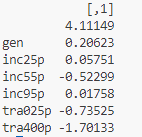
\includegraphics[width=0.2\textwidth]{5a.png}
    \caption{Coefficients from Newton's method}
\end{figure}
\item
\begin{figure}[h]
    \centering
    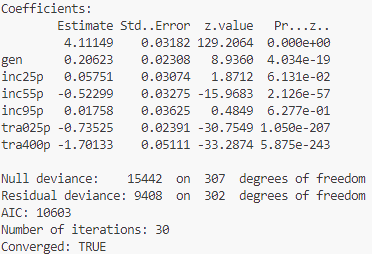
\includegraphics[width=0.5\textwidth]{5b.png}
    \caption{Summary of Newton's method}
\end{figure}

\begin{enumerate}
    \item Use of standard error assumes we are randomly and independently sampling from the population.
    \item Use of z value and p-value assumes the distribution is normal, and we know the population variance.
    \item Use of Null and residual deviance assumes the distribution is exponential and sample is independent. 
    \cite{npm}
    \item Use of AIC assumes the sample size is large and sample is independent and model estimates are from MLE
\end{enumerate}

\end{enumerate}

\newpage
\section*{Problem 6}
To get the loss function, We first remove the constant term \(\log(y!)\) from negative log-likelihood since it does not affect the optimization problem.
\begin{enumerate}[label=(\alph*)]
  \item 
  \begin{align*}
       \mathcal L(\beta_0 \vect \beta | \vectrm y, \vectrm X) &= \sum_{i=1}^{n} \left\{ [\beta_0 + \vect{\beta}^T \vectrm{x}_i]y_i -
            \exp\left\{\beta_0 + \vect{\beta}^T \vectrm{x}_i\right\}
            \right\} \\
  \end{align*}
Then we add the L2 regularization term to the loss function
  \begin{align*}
       \mathcal L_\lambda(\beta_0, \vect \beta | \vectrm y, \vectrm X) &= \sum_{i=1}^{n} \left\{ [\beta_0 + \vect{\beta}^T \vectrm{x}_i]y_i -
            \exp\left\{\beta_0 + \vect{\beta}^T \vectrm{x}_i\right\}
            \right\} + \lambda ||\vect \beta||_2^2
  \end{align*}

  We then derive the gradient and Hessian of the loss function

  \begin{align*}
    \frac{\partial}{\partial \beta_0} \mathcal L_\lambda(\beta_0, \vect \beta | \vectrm y, \vectrm X) &= -\sum_{i=1}^{n} y_i + \sum_{i=1}^{n}\exp(\beta_0 + \vect{\beta}^T \vectrm{x}_i) \\
    \frac{\partial}{\partial \vect{\beta}} \mathcal L_\lambda(\beta_0, \vect \beta | \vectrm y, \vectrm X) &= -\sum_{i=1}^{n} y_i \vectrm{x}_i + \sum_{i=1}^{n}\exp(\beta_0 + \vect{\beta}^T \vectrm{x}_i) \vectrm{x}_i - 2\lambda\vect \beta \\
    \frac{\partial^2}{\partial \beta_0^2} \mathcal L_\lambda(\beta_0, \vect \beta | \vectrm y, \vectrm X) &= \sum_{i=1}^{n}\exp(\beta_0 + \vect{\beta}^T \vectrm{x}_i) \\
    \frac{\partial^2}{\partial \vect{\beta}^2} \mathcal L_\lambda(\beta_0, \vect \beta | \vectrm y, \vectrm X) &= \sum_{i=1}^{n}\exp(\beta_0 + \vect{\beta}^T \vectrm{x}_i) \vectrm{x}_i \vectrm{x}_i^T - 2\lambda \vectrm I \\
    \frac{\partial^2}{\partial \beta_0 \partial \vect{\beta}} \mathcal L_\lambda(\beta_0, \vect \beta | \vectrm y, \vectrm X) &= \sum_{i=1}^{n}\exp(\beta_0 + \vect{\beta}^T \vectrm{x}_i) \vectrm{x}_i \\
  \end{align*}

  we can write the gradient and Hessian in matrix form as
  \begin{align*}
    \frac{\partial}{\partial \vect \beta'} \mathcal L_\lambda(\beta_0, \vect \beta, \vect \beta' | \vectrm y, \vectrm X) &= -\vectrm X^T \vectrm y
+ \vectrm X^T \exp(\vectrm X \vect \beta') - 2\lambda [0;\vect \beta] \\
    \frac{\partial^2}{\partial \vect \beta' \partial \vect \beta'^T} \mathcal L_\lambda(\beta_0, \vect \beta \vect \beta'| \vectrm y, \vectrm X) &= \vectrm X^T \diag(\exp \{\vectrm X \vect \beta'\}) \vectrm X - 2\lambda (\vectrm I - e_1e_1^T)
  \end{align*}

\item It is required that the Hessian matrix is positive definite for the loss function to be convex.
\item 
\newpage
\begin{figure}[h]
    \centering
    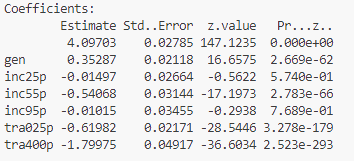
\includegraphics[width=0.5\textwidth]{6c.png}
    \caption{Coefficients from Regularized Newton's method}
\end{figure}
\item 
\begin{figure}[h]
    \centering
    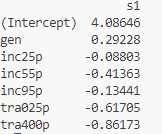
\includegraphics[width=0.5\textwidth]{6d.png}
    \caption{Coefficients from Regularized GLM}
\end{figure}

See (Appendix 6)

The coefficients from regularized Newton's method and regularized GLM are very close.
With \(\lambda = 10\), the tra400p coefficient is greatly increased, while the gen coefficient is slightly decreased. 

\end{enumerate}

\newpage
\section*{Problem 7}
\begin{enumerate}[label=(\alph*)]
  \item  See (Appendix 7)
  \item  See (Appendix 7)
  \item 

  \begin{figure}[h]
      \centering
      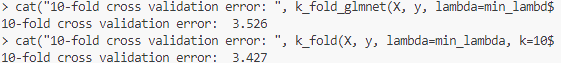
\includegraphics[width=0.5\textwidth]{7c.png}
      \caption{Compare Newton's method and GLM, both regularized with min lambda, first error is from GLM, second is from Newton's method}
  \end{figure}

  The regularized Newton's method has a lower error than the regularized GLM when the data is not randomized. When the data is randomized, the difference is undermined by the randomness.

\end{enumerate}

\newpage
\section*{Problem 8}
\begin{enumerate}[label=(\alph*)]
  \item  See (Appendix 8)
  \item  See (Appendix 8)
\end{enumerate}

\section*{Problem 9}
See (Appendix 9)
\begin{enumerate}[label=(\alph*)]
  \item 
  Let \(\hat{\beta}_0\) and \(\hat{\vect{\beta}}\) be the coefficients of the model obtained at the minimum of the cross-validation error.
  \[
  \E(y| \vectrm{x}_i) = \exp(\hat{\beta}_0 + \hat{\vect{\beta}}^T \vectrm{x}_i)
  \]
  \item  Yes, the regularization set the coefficients of inc25p and inc95p to 0 while keep the inc55p to be non-zero. This corresponds to the coefficients significance in 1a model where inc25p and inc95p are not significant.
  \item
  \begin{figure}[h]
      \centering
      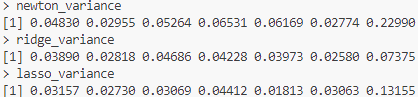
\includegraphics[width=0.5\textwidth]{q9c.png}
      \caption{Bootstrap CI}
  \end{figure}
  The approximated variances of coefficients from the bootstrapped regularized methods are lower than the variance from the MLE estimate. This is expected because the regularized methods penalize the coefficients more, which reduces the variance of the coefficients.
\end{enumerate}

\section*{Problem 10}
See (Appendix 10)
\begin{figure}[h]
    \centering
    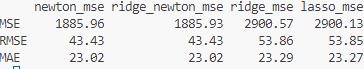
\includegraphics[width=0.5\textwidth]{10.png}
    \caption{MSE of different models}
\end{figure}

If we compare the Newton vs Ridge-Newton method, we can see that these two methods show remarkably similar performance with MSEs of ~2215.54 and 2215.38 respectively, and nearly identical RMSE and MAE values. This suggests that the ridge penalty in the Ridge-Newton method is having minimal impact on your model, possibly because
\begin{enumerate}
    \item The optimal regularization parameter is very small
    \item The features might not have high multicollinearity
    \item The dataset may be large enough relative to the number of features that regularization provides little benefit
\end{enumerate}

If we compare our regression with the glmnet's model, we can see that glmnet's model has a slightly lower MSE and RMSE where the lasso model is better than the ridge model in all metrics. This is expected because the optimization problem is the same for both methods.  \cite{Tay2023}

Now if we compare the PCA models with the non-PCA models, we can see that the PCA models have much lower MSE and RMSE than the non-PCA models. This is expected because the PCA completely removes the multicollinearity and noise in the data where both the ridge and lasso methods only mitigate the multicollinearity.




\newpage
\bibliography{refs}

\newpage
\section*{Appendix 1}
\inputminted{r}{q1.r}

\newpage
\section*{Appendix 2}
\inputminted{r}{q2.r}


\newpage
\section*{Appendix 5}
\inputminted{r}{q5.r}

\newpage
\section*{Appendix 6}
\inputminted{r}{q6.r}

\newpage
\section*{Appendix 7}
\inputminted{r}{q7.r}

\newpage
\section*{Appendix 8}
\inputminted{r}{q8.r}

\newpage
\section*{Appendix 9}
\inputminted{r}{q9.r}

\newpage
\section*{Appendix 10}
\inputminted{r}{q10.r}


\end{document}
